\section{Experimental Evaluation}
\label{sec:evaluation}
%\begin{comment}

This section aims to answer the following research questions: 

\begin{itemize}
\item \textbf{Effectiveness:} Whether \NP{} could detect more performance issues than existing NUMA-profilers? (Section~\ref{effectiveness}) How helpful is \NP{}'s report? (Section~\ref{sec:casestudies})
\item \textbf{Performance:} How much performance overhead is imposed by \NP{}'s detection, comparing to the state-of-the-art fine-grained tool? (Section~\ref{sec:performance}) 
\item \textbf{Memory Overhead:} What is the memory overhead of \sloppy \NP{}? (Section~\ref{sec:memory})
\item \textbf{Architecture Independence:} Whether \NP{} could detect the similar issues when running on a non-NUMA architecture? (Section~\ref{sec:archindependent})	
\end{itemize}

%\end{comment}

\textbf{Experimental Platform:}  \NP{} was evaluated on an Intel(R) Xeon(R) 8153 machine with 8 nodes and 128 physical cores in total, except in Section~\ref{sec:archindependent}. This machine is installed with 512GB of memory. Any two nodes in this machine are less than or equal to 3 hops, where the latency of two hops and three hops is 2.1 and 3.1 respectively, while the local latency is 1.0. The OS for this machine is Linux Debian 10 and the compiler is Clang-10.0.0 (LLVM).  The hyperthreading was turned off for the evaluation.
%\todo{Xin: could you find out the toplogy of the machine? such as adding a figure about how different nodes are connected together (how many hops). }

%\todo{Xin: make sure that all performance numbers, issue numbers are correct (because you have changed the case number). } 

\subsection{Effectiveness}
\label{effectiveness}
%%\renewcommand{\arraystretch}{1.5}
\begin{table}[!htp]
% \footnotesize
% \setlength{\tabcolsep}{0.3em}
  \centering
    \begin{tabular}{|l|r|}
    \hline
    \multirow{1}{*}{Issue Categories}&Score \\ \hline
    \PS&1500\\ \hline
    \FS&100\\ \hline
    \TS&100\\ \hline
    \TM&150\\ \hline
    \end{tabular}
  \caption{Score threshold for different categories of issues.
  \label{tab:memory_consumption}}
\end{table}
%\renewcommand{\arraystretch}{1.5}
\begin{table*}[tp]
%\footnotesize
% 	\setlength{\tabcolsep}{0.3em}
\centering
\begin{tabular}{|l|c|l|r|l|r|r|c|c|}
    \hline
    \cline{1-8}
    \multirow{2}{*}{Application}& \multirow{2}{*}{Improve}& \multicolumn{5}{c}{Specific Issues}&\\
    \cline{3-8}
    & & Issue & Score & \multicolumn{1}{|c|}{Allocation Site} & \multicolumn{1}{|c|}{Fix Strategy} & Improve & New \\ 
    \hline 
    % Application & Issue (score) & Strategy&New&Source Code&RunningTime&Final RunningTime\\ \hline
    
    \multirow{2}{*}{AMG2006}&\multirow{2}{*}{160\%}&\PS&3612&par\_rap.c:1385&\BI&160\%& \\
    \cline{3-8}
    
    &&\TM&230&&\TB&132\%&\checkmark \\ \hline

    \multirow{7}{*}{lulesh}&\multirow{7}{*}{594\%}&\PS&1978&lulesh.cc:543-545&\BI&429\%& \\
    \cline{3-8}

    &&\PS&1611&lulesh.cc:1029-1034&\BI&504\%&  \\
    \cline{3-8}
    
    &&\PS&1283&\multirow{2}{*}{lulesh.cc:2251-2264}&\BI&\multirow{2}{*}{416\%}& \\
    &&\FS&174&& + \PAD && \checkmark\\
    \cline{3-8}
    
    &&\PS&1316&\multirow{2}{*}{lulesh.cc:2089}&\BI&\multirow{2}{*}{391\%}& \\
    &&\FS&170&& + \PAD && \checkmark\\
    \cline{3-8}
    
    &&\TM&153&&\TB&382\%&\checkmark \\ \hline
    
    UMT2013&131\%&\TM&253&&\TB&131\%&\checkmark \\
    \hline 
    \hline
    
    bodytrack&105\%&\TM&13646&&\TB&105\% &\checkmark \\ \hline
    
    dedup&106\%&\TI&&& adjust threads assignment &106\%&\checkmark \\ \hline
    
    facesim&105\%&\TM&399&&\TB&105\%&\checkmark \\ \hline
    
    ferret&208\%&\TI&&& adjust threads assignment &208\%&\checkmark \\ \hline
 
    \multirow{5}{*}{fluidanimate}&\multirow{5}{*}{429\%}&\PS&154&\multirow{2}{*}{pthreads.cpp:294}&\PI&\multirow{2}{*}{150\%}& \\
    &&\FS&223&& + \PAD&&\checkmark \\
    \cline{3-8}
    
    &&\PS&45994&\multirow{2}{*}{pthreads.cpp:292}& \multirow{2}{*}{\PI} &\multirow{2}{*}{340\%}& \\
    &&\TS&19545&&&&\checkmark \\
    \cline{3-8}
     
    &&\TM&812&&\TB&418\%&\checkmark \\ \hline
    
    \multirow{4}{*}{streamcluster}&\multirow{4}{*}{167\%}&\PS&405&\multirow{2}{*}{streamcluster.cpp:984}&\PI&\multirow{2}{*}{105\%}& \\
    &&\FS&368&& + \PAD&& \checkmark\\
    \cline{3-8}
     
    &&\PS&6397&streamcluster.cpp:1845&\DUP&158\%& \\
    \cline{3-8}
     
    &&\TM&252&&\TB&132\%&\checkmark \\ \hline
    \end{tabular}
  \caption{Detected NUMA performance issues of \NP{}, where it detects multiple performance bugs that cannot be detected using existing NUMA profilers (with a check mark in the last column). \todo{Differentiate the performance impact caused by false sharing and page sharing}}
  \label{tab:numa_issues}
\end{table*}



We evaluated \NP{} on multiple HPC applications (e.g., \sloppy AMG2006~\cite{AMG2006}, lulesh~\cite{LULESH}, and UMT2013~\cite{UMT2013}) and a widely-used multithreaded application benchmark suite --- PARSEC~\cite{parsec}.  Applications with NUMA performance issues are listed in Table~\ref{tab:numa_issues}. The ``Improve'' column of Table~\ref{tab:numa_issues} also shows the performance improvement (the average of 10 executions) after fixing the corresponding issue based on the tool's feedback. Here, the basic version is running with the default \texttt{glibc} library  without thread binding. We divide the runtime of this basic version by the runtime after fixes to get the improvement rate. For each issue, the table listed the type of issue and the corresponding score (if applicable), the allocation site, and the fix strategy. Note that the table only shows cases with  page sharing scores larger than 1500 (if without cache false/true sharing), false/true sharing scores larger than 1, and thread migration scores larger than 150. Further, the performance improvement of each specific issue is listed as well. We also present multiple case studies that show how helpful is \NP{}'s report in Section~\ref{sec:casestudies}.   

Overall, we have the following observations. First, it reports no false positives by only reporting scores larger than the above-mentioned thresholds. Second, \NP{} 
detects more performance issues than the combination of all existing NUMA profilers~\cite{Intel:VTune, Memphis, Lachaize:2012:MMP:2342821.2342826, XuNuma, NumaMMA, 7847070, diener2015characterizing, valat:2018:numaprof}. The performance issues that cannot be detected by existing NUMA profilers are highlighted with a checkmark in the last column of the table, although some can be detected by other  tools (but not NUMA tools), such as cache false/true sharing issues~\cite{Sheriff, Predator, Cheetah, DBLP:conf/ppopp/ChabbiWL18, helm2019perfmemplus}. This comparison with existing NUMA profilers is based on the methodology, instead of based on the results of specific tools. Some difficulties exist for the direct comparison. For instance, although  NUMAPROF can run successfully on our machine~\cite{valat:2018:numaprof}, it is  difficult to compare with directly due to the following reasons: (1) it does not provide the data-centric view and only reports statements with remote accesses. This shortcoming makes it difficult to identify the issue. (2) Further, NUMAPROF does not use a threshold-based approach, which may report a lot of statements with a small number of remote accesses. Thus, it is difficult to utilize the reports of NUMAPROF directly. \NP{} overcomes these issues by only reporting issues with high impacts, relying on a set of new metrics. Therefore, if an issue is labeled as ``\checkmark'' in the ``New'' column in Table~\ref{tab:numa_issues}, this issue is definitely not detectable by all existing NUMA profilers from the methodology point of view. Overall, existing NUMA profilers cannot detect false or true sharing and issues caused by thread migration and load imbalance. 
%Note that false sharing or true sharing issues, as well as thread imbalance issues, can be detected using specific tools, but cannot be detected by existing NUMA profilers. That is the reason why they are still labelled as ``New'' in the table. 

When comparing to a specific profiler, \NP{} also has better results even on detecting remote accesses. For lulesh, HPCToolkit only detects issue \# 4~\cite{XuNuma}, while \NP{} detects three more issues (\# 3, 5, 7) additionally . Fixing these issues improves the performance by up to 504\% (e.g., \# 3). Multiple reasons may contribute to this big difference. 
First, \NP{}'s predictive method is able to  detect issues that are not occurred in the current scheduling and the current hardware, while HPCToolkit has no such capabilities. Second, HPCToolkit requires binding threads to nodes, which may miss remote accesses caused by its specific binding. 
Third, \NP{}'s fine-grained profiling provides  better effectiveness than a coarse-grained profiler like HPCToolkit. 
\NP{} may have false negatives caused by its instrumentation. \NP{} cannot detect an issue (\# 11 in Table~\ref{tab:numa_issues}) of UMT2013 reported by HPCToolkit~\cite{XuNuma}. The basic reason is that \NP{} (inherited from LLVM) cannot compile Fortran code successfully. \NP{}'s limitations are further discussed in Section~\ref{sec:casestudies}.



\subsection{Case Studies}
\label{sec:casestudies}
In this section, multiple case studies are shown how programmers could fix performance issues based on the report. 
\lstset{ %
backgroundcolor=\color{white},      % choose the background color
basicstyle=\footnotesize\ttfamily,  % size of fonts used for the code
columns=fullflexible,
tabsize=4,
breaklines=true,               % automatic line breaking only at whitespace
captionpos=b,                  % sets the caption-position to bottom
commentstyle=\color{mygreen},  % comment style
escapeinside={\%*}{*)},        % if you want to add LaTeX within your code
keywordstyle=\color{blue},     % keyword style
stringstyle=\color{mymauve}\ttfamily,  % string literal style
frame=single,
rulesepcolor=\color{red!20!green!20!blue!20},
% identifierstyle=\color{red},
language=c++,
}



\subsubsection{Remote Accesses}

For remote accesses, \NP{}  not only reports remote access scores, indicating the seriousness of the corresponding issue, but also provides additional information to reduce remote accesses. Remote accesses can be reduced with different strategies, such as padding (false sharing), block-wise interleaving~\cite{XuNuma}, duplication, and page interleaving. Block-wise interleaving is to divide the whole object into multiple blocks, and then bind each block and threads accessing it to the corresponding NUMA node.  

\NP{} provides a data-centric analysis, as existing work~\cite{XuNuma}. That is, it always attributes performance issues to its allocation callsite. \NP{} also shows the seriousness with its remote access score. 

\NP{} further reports more specific information to guide the fix. As shown in Listing~\ref{blockinterleave} (\#5), \NP{} further reports each page that is accessed by which threads. Based on this information,  block-wise interleaving is a better strategy for the fix, which achieves a better performance result. However, for Issue \# 18 or \# 20 of \texttt{fluidanimate}, there is no such access pattern. Therefore, these issues can be fixed with the normal page interleave method. 

%\XZ{remote score and false sharing score are fixed. What is the case number?You mean issue number? is not used.}
\begin{lstlisting}[caption={Remote access issue of lulesh },label={blockinterleave},captionpos=b]
Allocation Site: lulesh.cc:2251
Remote score:  1220
False sharing score:  13
True Sharing score:   0.00
Pages accessed by threads:
    0--8, 8--16, 16--23, 23--31 ......
\end{lstlisting}
%\todo{I didn't find lulesh.cc:2251 has an issue. I also didn't find the score. Make sure the score is the same as Table 1 and Table 3}. 

%\todo{Sorry, do not have time to do this. Better to check if we don't use duplications, how much performance we can achieve for this example. But this is in lower priority} 
Listing~\ref{duplicate} shows another example of remote accesses. For this issue (\# 25), a huge number of continuous reads (2330M) were detected after the last write. Based on such a report, the object can be duplicated to different physical nodes, which improves the performance by 158\%, which achieves significantly better performance than page interleaving.

\NP{} differentiates cache coherency issues from normal remote accesses, and further differentiates false sharing from true sharing due to different fix strategies. Given the report, programmers could utilize the padding to eliminate false sharing issues. As shown in Table~\ref{sec:evaluation}, many issues have false sharing issues (e.g., \#6, \#8, \#13, \#21, \#24). Fixing them with the padding could easily boost the performance, which cannot be done without the detailed report. Instead, true sharing will utilize a different fix strategy, such as page interleaving. Overall, \NP{}'s precise report provides better information to guide the fixes.  
\begin{lstlisting}[caption={Remote access issue of streamcluster},label={duplicate},captionpos=b]
Allocation site:streamcluster.cpp:1845
Remote score:   7169
False sharing score:  0.00
True Sharing score:   0.00
Continuous reads after the last write:   2443582804
\end{lstlisting}

%However a further interleaved strategy could give more benefits after padding as showed in Table~\ref{sec:evaluation} for Issue[5,7,11,19,22].But true sharing is very hard to be eliminated, so a simple interleaved strategy is applied for Issue[18] in Table~\ref{sec:evaluation} to reduce resource contention for NUMA architecture. 

\subsubsection{Thread Migration} 
%\todo{xin new writing
When an application has frequent thread migrations, it may introduce excessive thread migrations. For such issues, the fix strategy is to bind threads to nodes. Typically, there are two strategies: round-robin and packed binding. Round robin is to bind continuous threads to different nodes one by one,  ensuring that different nodes have a similar number of threads. Packed binding is to bind multiple threads to the first node, typically the same as the number of hardware cores in one node, and then to another node afterward. Based on our observation, round-robin typically achieves a better performance than packed binding, which is the default binding policy for our evaluations in Table~\ref{tab:numa_issues}. Thread binding itself achieves a good performance improvement (e.g., 418\% for \texttt{fluidanimate}), which indicates the importance of binding for some applications. 

%Listing~\ref{blockinterleave} 

%For \NP{}  to help users to pick a better one. For example, in , packed binding could give further benefits combined with block-wise interleaved, since it not only could eliminate contention to the memory controller, but also could make most remote memory access turned into local access. On the other hand, if no such memory access pattern is found, users could just pick anyone. In our experiments, round-robin is picked by default.
%}
%\todo{Thread migration can be fixed with thread binding. There are two ways of binding: packed binding or round-robin binding? Can \NP{} tells us what type of binding will provide better performance? }

\subsubsection{Load Imbalance}

For load imbalance, \NP{} not only reports the existence of such issues but also suggests a thread assignment that could help reduce these issues. As discussed in Section~\ref{sec:loadimbalance}, \NP{} predicts the assignment based on the number of sampled memory accesses: \textit{the number of threads for each type should have a similar proportion as the number of memory accesses from each type of threads}. That is, if two type
of threads has a one-to-two proportion on memory accesses, then the number of threads should also follow this one-to-two proportion. 

For \texttt{dedup}, \NP{} reports that memory accesses of anchor, chunk, and compress threads have a proportion of $92.2:0.33:3.43$, when all libraries are instrumented and the total number is set to 96. By checking the code, we found that \textttt{dedup} actually employs a pipeline model with five stages, including  dataprocess, anchor, chunk,  compress, and sendblock, but the number of threads for both dataprocess and sendblock stages has been set to 1 in the code.  Based on the reported number, the portion of the chunk and compress threads should be around 1 to 10. However, setting the threads to be 1 may introduce high contention, since producers and consumers are sharing the same lock. Instead, we set the number of chunk threads to be 2, and further set the number of compress threads to be 18, and the number of anchor threads to be 76. 
%The corresponding queues are \todo{18:2:2:4 (76:18:2??)} \XZ{this is the proportion of the queue.But maybe need Jin's help to explain how to get this. }
With this setting, \texttt{dedup}'s performance is improved by 16\%. We further compare its performance with the suggested assignment of another existing work--SyncPerf~\cite{SyncPerf}. SyncPerf assumes that different types of threads should have the same waiting time. SyncPerf proposes the best assignment should be $24:24:48$, which could only improve the performance by 5\%. 
%That is, \NP{}'s suggestion is much better than SyncPerf's suggestion for load imbalance issue. 

For another example---\texttt{ferret}, \NP{} suggests a proportion of $3.3 :1.9 :47.4 :75.3$ for its four types of threads. With this suggestion, we are configuring the threads to be $4 : 2 : 47 : 75$. With this assignment, \texttt{ferret}'s performance increases by 106\% compared with the original version. In contrast, SyncPerf suggests an assignment of $1:1:2:124$
. However, employing this assignment actually degrades the performance by 354\% instead. 

Overall, \NP{} suggested optimal assignment for load imbalance issues achieves the better performance than SyncPerf~\cite{SyncPerf}. 
%We don't know the exact reason why SyncPerf fails to predict the optimal assignment,

\subsection{Performance Overhead}
\label{sec:performance}
\begin{figure}[!h]
    \centering
    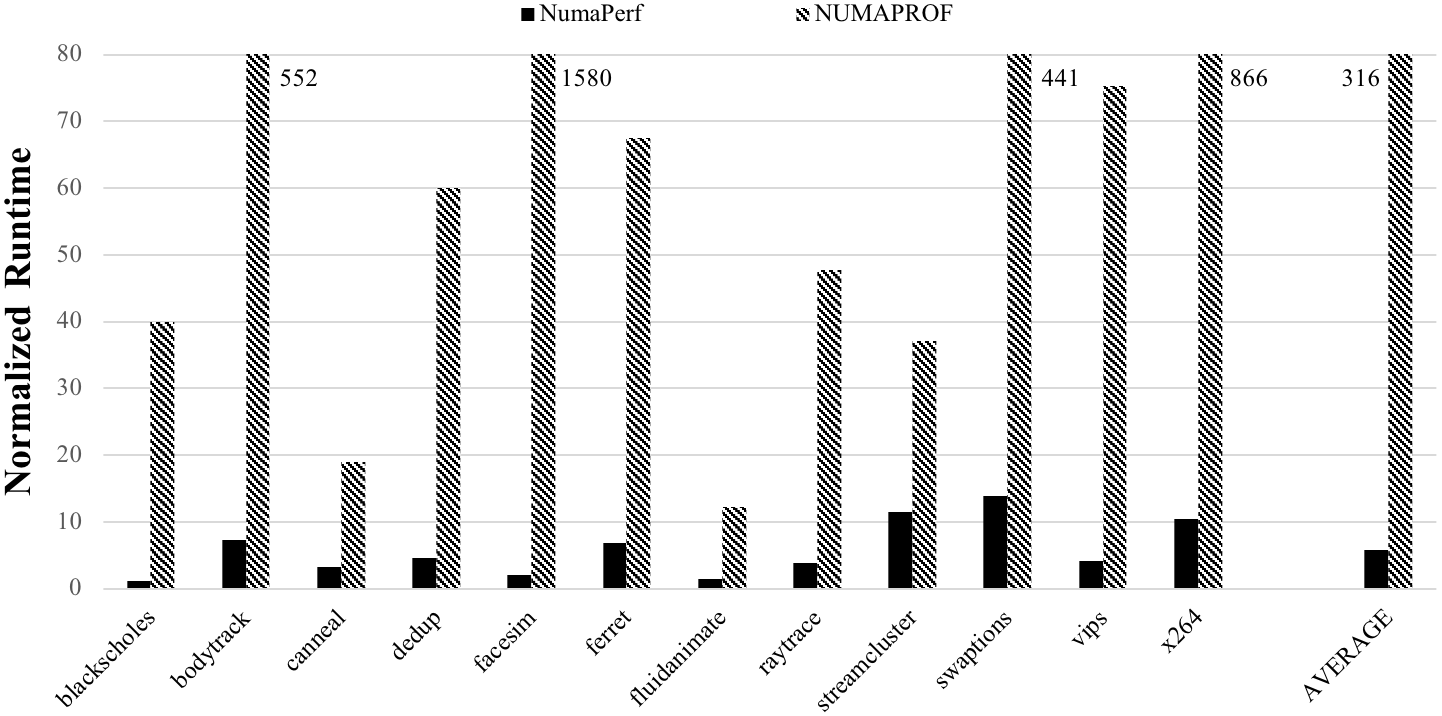
\includegraphics[width=3.2in]{paper/figures/performance.pdf}
    \caption{Performance overhead of \NP{} and others.\label{fig:performance}}  
\end{figure}


We also evaluated the performance overhead of \NP{} on PARSEC applications, as shown in Figure~\ref{fig:performance}. On average, \NP{}'s overhead is around 585\%, which is orders-of-magnitude smaller than the state-of-the-art fine-grained profiler --- NUMAPROF~\cite{valat:2018:numaprof}. In contrast, NUMAPROF's overhead runs $316\times$ slower than the original one. \NP{} is designed carefully to avoid such high overhead, as discussed in Section~\ref{sec:implementation}. Also, \NP{}'s compiler-instrumentation also helps reduce some overhead, such as excluding memory accesses on stack variables. 

There are some exceptions with high overhead. Two applications impose more than $10\times$ overhead, including \texttt{swaptions} and \texttt{x264}. Based on our investigation, the instrumentation with an empty function imposes more than $5\times$ overhead for both applications. The reason is that they have significantly more  memory accesses compared with other applications like \texttt{blackscholes}. Based on our investigation, \texttt{swaptions} has more than $250\times$ memory accesses than \texttt{blackscholes} for the same time unit. Applications with lower overhead are those ones where many accesses come from non-instrumented components, e.g., libraries. 

%Besides, \NP{} has to do lots of computation inside the intercepting function which could make memory access go up to multiple times. And if a target application contains any NUMA issues, the issue also could arise in \NP{}. Based on this situation, we believe \NP{} did it very well to achieve a good performance. 

\subsection{Memory Overhead}
\label{sec:memory}
%\renewcommand{\arraystretch}{1.5}
\begin{table}[!htp]
% \footnotesize
% \setlength{\tabcolsep}{0.3em}
  \centering
    \begin{tabular}{|l|r|r|r|}
    \hline
    \multirow{2}{*}{Apps}&
    \multicolumn{3}{c|}{Memory Usage (MB)}\\
    \cline{2-4}
    &Glibc&\NP&NUMAPROF \\ \hline
    \hline
    blackscholes&617&689&685\\ \hline
    bodytrack&36&139&260\\ \hline
    canneal&887&1476&2383\\ \hline
    dedup&917&1806&2388\\ \hline
    facesim&2638&2826&3005\\ \hline
    ferret&160&301&445\\ \hline
    fluidanimate&470&667&753\\ \hline
    raytrace&1287&1610&2089\\ \hline
    streamcluster&112&216&928\\ \hline
    swaptions&28&67&255\\ \hline
    vips&226&283&463\\ \hline
    x264&2861&3039&3108\\ \hline \hline  
    Total&{\bf 10238}&{\bf 13120}&{\bf 16762}\cr\hline
    \end{tabular}
  \caption{Memory consumption of different profilers. \label{tab:memory_consumption}}
  \vspace{-0.2in}
\end{table}

We further evaluated \NP{}'s memory overhead with PARSEC applications. The results are shown in Table~\ref{tab:memory_consumption}. In total, \NP{}'s memory overhead is around 28\%, which is  smaller than the state-of-the-art fine-grained profiler --- NUMAPROF~\cite{valat:2018:numaprof}. \NP{}'s memory overhead is mainly coming from the following resources. First, \NP{} records the detailed information in page-level and cache-level, so that we could provide detailed information about these issues. Second, \NP{} also stores allocation callsites for every object in order to attribute performance issues back to the data. 

We notice that some applications have a larger percentage of memory overhead, such as \texttt{streamcluster}. For this object, a large object has a very serious NUMA issue. Therefore, recording page and cache level detailed information contributes to the major memory overhead. However, overall, \NP{}'s memory overhead is totally acceptable, since it provides much more helpful information. 

%and thread based levels, especially \NP{} also provides lots of help information to help users fix the issues.
%Because \NP{} has to use lots of memory to record variety memory access patterns in all levels for potential issues. That is why some applications like bodytrack, dedup and streamcluster could get 2 times memory overheads.In these applications, they got some very huge objects with very serious NUMA issues ,like streamcluster contained an object that could occupy 100MB.To track the access pattern and provide detailed help information, doubled or more memory overheads are very reasonable.So to reduce memory overheads, \NP{} applied lots of mechanisms to avoid some objects if they look like not suspicious.That is why some applications like blackscholes, facesim and x264 bring very tiny memory overheads.Overall, \NP{} occupied less memory compared with NUMAPROF, but provided more information.

%\todo{Adding some explanation for memory utilization}. 

\subsection{Architecture Sensitiveness}
\label{sec:archindependent}

We further confirm whether \NP{} is able to detect similar performance issues when running on a non-NUMA or UMA machine. We further performed the experiments on a two-processor machine additionally, where each processor is Intel(R) Xeon(R) Gold 6230 and each processor has 20 cores. We explicitly disabled all cores in node 1 but only utilizing 16 hardware cores in node 0, in order to avoid the NUMA effect. This machine has 256GB of main memory, 64KB L1 cache, and 1MB of L2 cache. The experimental results are further listed in Table~\ref{tab:independent}. For simplicity, we only listed the applications, the issue number, and serious scores in two different machines. 

Table~\ref{tab:independent} shows that most reported scores in two machines are very similar, but with small variances. The small variances could be caused by multiple factors, such as parallelization degree (concurrency). However, this table shows that all serious issues can be detected on both machines. This indicates that \NP{} achieves its design goal, which could even detect NUMA issues without running on a NUMA machine. 

% \begin{table}[!htp]
% %\footnotesize
%  	\setlength{\tabcolsep}{0.3em}
% \centering
% \begin{tabular}{|c|l|l|r|r|}
%     \hline
%     \cline{1-5}
%     \multirow{2}{*}{Application}& \multicolumn{4}{c}{Specific Issues}\\
%     \cline{2-5}
%     & \# & Type & \multicolumn{1}{|c|}{\specialcell{Score\\(NUMA)}}  & \multicolumn{1}{|c|}{\specialcell{Score\\(UMA)}}\\ \hline

%     \multirow{2}{*}{AMG2006} & 1 & \PS & & \\
%     \cline{2-5}
    
%     &  2 &\TM&230 &\\ \hline

%     \multirow{7}{*}{lulesh}& 3 &\PS&1978&  \\
%     \cline{2-5}

%     &4&\PS&1611 &  \\
%     \cline{2-5}
    
%     &&5&\PS&1283&\multirow{2}{*}{lulesh.cc:2251-2264}&\BI&406\%&\multirow{2}{*}{418\%}& \\
%     \cline{3-5}\cline{7-8}\cline{10-10}
%     &&6&\FS&174&&\PAD &403\%&& \checkmark\\
%     \cline{3-10}
    
%     &&7&\PS&1316&\multirow{2}{*}{lulesh.cc:2089}&\BI&392\%&\multirow{2}{*}{407\%}& \\
%     \cline{3-5}\cline{7-8}\cline{10-10}
%     &&8&\FS&170&&\PAD &402\%&& \checkmark\\
%     \cline{3-10}
    
%     &&9&\TM&153&&\TB&\multicolumn{2}{|c|}{382\%}&\checkmark \\ \hline
    
%     UMT2013&131\%&10&\TM&253&&\TB&\multicolumn{2}{|c|}{131\%}&\checkmark \\
%     \hline 
%     \hline
    
%     \multirow{3}{*}{bodytrack}&\multirow{3}{*}{109\%}&11&\PS&10444&\multirow{2}{*}{FlexImageStore.h:146}&\PI&\multicolumn{2}{|c|}{\multirow{2}{*}{106\%}}& \\
%     \cline{3-5}\cline{7-7}\cline{10-10}
%     &&12&\FS&328&& &\multicolumn{2}{|c|}{}&\checkmark \\
%     \cline{3-10}
%     &&13&\TM&13646&&\TB&\multicolumn{2}{|c|}{105\%}&\checkmark \\ \hline
    
%     dedup&116\%&14&\TI&&& adjust threads  &\multicolumn{2}{|c|}{116\%}&\checkmark \\ \hline
    
%     facesim&105\%&15&\TM&399&&\TB&\multicolumn{2}{|c|}{105\%}&\checkmark \\ \hline
    
%     ferret&206\%&16&\TI&&& adjust threads  &\multicolumn{2}{|c|}{206\%}&\checkmark \\ \hline
 
%     \multirow{5}{*}{fluidanimate}&\multirow{5}{*}{429\%}&17&\PS&154&\multirow{2}{*}{pthreads.cpp:294}&\PI&112\%&\multirow{2}{*}{160\%}& \\
%     \cline{3-5}\cline{7-8}\cline{10-10}
%     &&18&\FS&223&&\PAD&158\%&&\checkmark \\
%     \cline{3-10}
    
%     &&19&\PS&45994&\multirow{2}{*}{pthreads.cpp:292}& \multirow{2}{*}{\PI} &\multicolumn{2}{|c|}{\multirow{2}{*}{340\%}}& \\
%     \cline{3-5} \cline{10-10}
%     &&20&\TS&19545&&&\multicolumn{2}{|c|}{}&\checkmark \\
%     \cline{3-10}
     
%     &&21&\TM&812&&\TB&\multicolumn{2}{|c|}{418\%}&\checkmark \\ \hline
    
%     \multirow{4}{*}{streamcluster}&\multirow{4}{*}{167\%}&22&\PS&405&\multirow{2}{*}{streamcluster.cpp:984}&\PI&100\%&\multirow{2}{*}{103\%}& \\
%     \cline{3-5}\cline{7-8}\cline{10-10}
%     &&23&\FS&368&&\PAD&102\%&& \checkmark\\
%     \cline{3-10}
     
%     &&24&\PS&6397&streamcluster.cpp:1845&\DUP&\multicolumn{2}{|c|}{158\%}& \\
%     \cline{3-10}
     
%     &&25&\TM&252&&\TB&\multicolumn{2}{|c|}{132\%}&\checkmark \\ \hline
%     \end{tabular}
%   \caption{Detected NUMA performance issues of \NP{}, where it detects 15 performance bugs that cannot be detected using existing NUMA profilers (with a check mark in the last column).}
%   \label{tab:independent}
% \end{table}

%\todo{Can not run UMT2013 successfully in UMA after a lot of efforts, need more time to fix}

\begin{table}[!htp]
%\footnotesize
 	\setlength{\tabcolsep}{0.45em}
\centering
\begin{tabular}{|c|l|l|l|l|}
\hline
\multirow{2}{*}{Application}  & \multicolumn{4}{c|}{Specific   Issues}                                                              \\ \cline{2-5} 
                              & \# & \multicolumn{1}{c|}{Type} & \multicolumn{1}{c|}{\specialcell{Score\\(NUMA)}} & \multicolumn{1}{c|}{\specialcell{Score\\(UMA)}} \\ \hline
\multirow{2}{*}{AMG2006}       & 1  & \PS     & 7390  & 5405  \\ \cline{2-5} 
                               & 2  & thread migration & 6     & 6      \\ \hline
\multirow{7}{*}{lulesh}        & 3  & \PS     & 1840  & 2443  \\ \cline{2-5} 
                               & 4  & \PS     & 1504  & 2353  \\ \cline{2-5} 
                               & 5  & \PS     & 4496  & 4326  \\ \cline{2-5} 
                               & 6  & false sharing    & 26    & 51   \\ \cline{2-5} 
                               & 7  & \PS     & 1229  & 2136  \\ \cline{2-5} 
                               & 8  & false sharing    & 12    & 27    \\ \cline{2-5} 
                               & 9  & thread migration & 3328  & 5213      \\ \hline
UMT2013                        & 10 & thread migration & 18    &      \\ \hline \hline
\multirow{3}{*}{bodytrack}     & 11 & \PS     & 10800 & 8203  \\ \cline{2-5} 
                               & 12 & false sharing    & 24    & 153   \\ \cline{2-5} 
                               & 13 & thread migration & 297   & 190   \\ \hline 
dedup                          & 14 & thread imbalance &   92:1:3    &  88:4:4     \\ \hline
facesim                        & 15 & thread migration & 607   & 274   \\ \hline
ferret*                          & 16 & thread imbalance &      &       \\ \hline
\multirow{5}{*}{fluidanimate} & 17 & \PS              & 90534                            & 15765 \\ \cline{2-5} 
                               & 18 & true sharing     & 2941  & 1753  \\ \cline{2-5} 
                               & 19 & \PS     & 180   & 95   \\ \cline{2-5} 
                               & 20 & false sharing    & 20    & 80    \\ \cline{2-5} 
                               & 21 & thread migration & 73    & 34    \\ \hline
\multirow{4}{*}{streamcluster} & 22 & \PS     & 427   & 270   \\ \cline{2-5} 
                               & 23 & false sharing    & 31    & 153   \\ \cline{2-5} 
                               & 24 & \PS     & 7169  & 10259 \\ \cline{2-5} 
                               & 25 & thread migration & 229   & 214   \\ \hline
\end{tabular}
  \caption{Evaluation on architecture Sensitiveness. We evaluated \NP{} on a non-NUMA (UMA) machine, which has very similar results as that on a NUMA machine. For \texttt{ferret}, \NP{} reports a proportion of  $3:2:48:75$ on the 8-node NUMA machine, and $5:4:50:77$ on the UMA machine. \label{tab:independent}}
  \vspace{-0.2in}
\end{table}




